\documentclass[lualatex]{beamer}
\usepackage[english]{babel}
\usepackage{graphicx}
\usepackage{minted}

\setbeameroption{show notes}
\usetheme{Madrid}
\definecolor{codebg}{rgb}{0.9,0.9,0.9}
\setminted{autogobble,bgcolor=codebg,fontsize=\footnotesize}%fontfamily=Inconsolata,

\title[Errors]{A Very Short Summary to Error Handling}
  \author{Taoda}
  \institute{YITU tech}
  \date{Jan.\ 2018}

\begin{document}

\begin{frame}
\titlepage
\end{frame}

\begin{frame}
  \frametitle{Outline}
  \tableofcontents
\end{frame}

\section{Terminology}

\begin{frame}
  \frametitle{What is an error?}
  \begin{block}{~}
    \begin{itemize}
    \item Error: \textcolor{blue}{expected} inputs, prematurely stopping the execution.
    \item Panic: \textcolor{blue}{unexpected} inputs, prematurely stopping the execution.
    \item Assertion: a predicate, which must hold at that point in every execution, triggers a panic when fails.
    \end{itemize}
  \end{block}
\end{frame}

\section{Return code}

\begin{frame}[fragile]
  \frametitle{Return code}

  \begin{minted}{c}
    int r = system("/bin/ls");
    if (r != 0) goto fail;
  \end{minted}

  \begin{block}{Dark side}
    \begin{itemize}
    \item No details.
    \item Hard to maintain return codes universally.
    \item Boilerplate error handling code.
    \item Return code will implicitly be ignored.
    \end{itemize}
  \end{block}
\end{frame}

\section{The Rise of Exception}

\begin{frame}[fragile]
  \frametitle{The Rise of Exception: Exception}

  \begin{minted}{cpp}
    try {
      doSomething();
    } catch(const std::exception& ex) {
      handleError(ex);
    }
  \end{minted}

  \begin{block}{Good part}
    \begin{itemize}
    \item Object-oriented
      \begin{itemize}
      \item Details can be stored in exception objects.
      \item Type hierarchy of exceptions must be defined, in some extent, universally.
      \end{itemize}
    \item Stack unwinding
      \begin{itemize}
      \item Eliminates the pass-the-hand code.
      \item Once implicitly ignored, the entire program will be crashed.
      \end{itemize}
    \end{itemize}
  \end{block}
\end{frame}

\begin{frame}[fragile]
  \frametitle{The Rise of Exception: Exception}

  \begin{minted}{cpp}
    try {
      doSomething();
    } catch(...) {
      LOG("something bad happened.");
      throw;
    }
  \end{minted}

  \begin{alertblock}{~}
    \begin{itemize}
    \item Aimless catching: Catching must be specific. Do never catch anything you don't understand.
    \end{itemize}
  \end{alertblock}
\end{frame}

\begin{frame}
  \frametitle{The Rise of Exception: Checked Exception}

  \begin{block}{Checked Exception}
    Exceptions that a method may raise are part of the method's signature.
  \end{block}
\end{frame}

\begin{frame}[fragile]
  \frametitle{The Rise of Exception: Checked Exception}

  \begin{minted}{java}
    interface Something {
      void f() throws Throwable;
    }
  \end{minted}

  \begin{alertblock}{~}
    Checked exception is a way to handle errors, rather than panics.
  \end{alertblock}
\end{frame}

\begin{frame}[fragile]
  \frametitle{The Rise of Exception: Checked Exception}

  \begin{minted}{java}
    interface Something {
      void f() throws Exception;
    }
  \end{minted}

  \begin{alertblock}{~}
    Aimless throwing: Throwing too general type of exceptions, with which users know little to deal.
  \end{alertblock}
\end{frame}

\begin{frame}[fragile]
  \frametitle{The Rise of Exception: Checked Exception}

  \begin{minted}{java}
    public static Object unserialize(byte[] bytes)
        throws IOException, ClassNotFoundException {
        try (ByteArrayInputStream bais = new ByteArrayInputStream(bytes)) {
            ObjectInputStream ois = new ObjectInputStream(bais);
            return ois.readObject();
        }
    }
  \end{minted}

  \begin{alertblock}{~}
    Exception passing-through: Pass exceptions through boundaries of abstraction.
  \end{alertblock}
\end{frame}

\section{The Fall of Exception}

\begin{frame}
  \frametitle{The Fall of Exception}

  \begin{block}{Criticism on checked exception}
    The throws clause, at least the way it's implemented in Java, doesn't necessarily force you to handle the exceptions,
    but if you don't handle them, it forces you to acknowledge precisely which exceptions might pass through.
    It requires you to either catch declared exceptions or put them in your own throws clause.
    To work around this requirement, people do ridiculous things.
    For example, they decorate every method with, "throws Exception."
    That just completely defeats the feature, and you just made the programmer write more gobbledy gunk.
    That doesn't help anybody.

    \hfill --- Anders Hejlsberg
  \end{block}
\end{frame}

\begin{frame}
  \frametitle{The Fall of Exception}
  \begin{block}{The Rise of Asynchronous IO}
    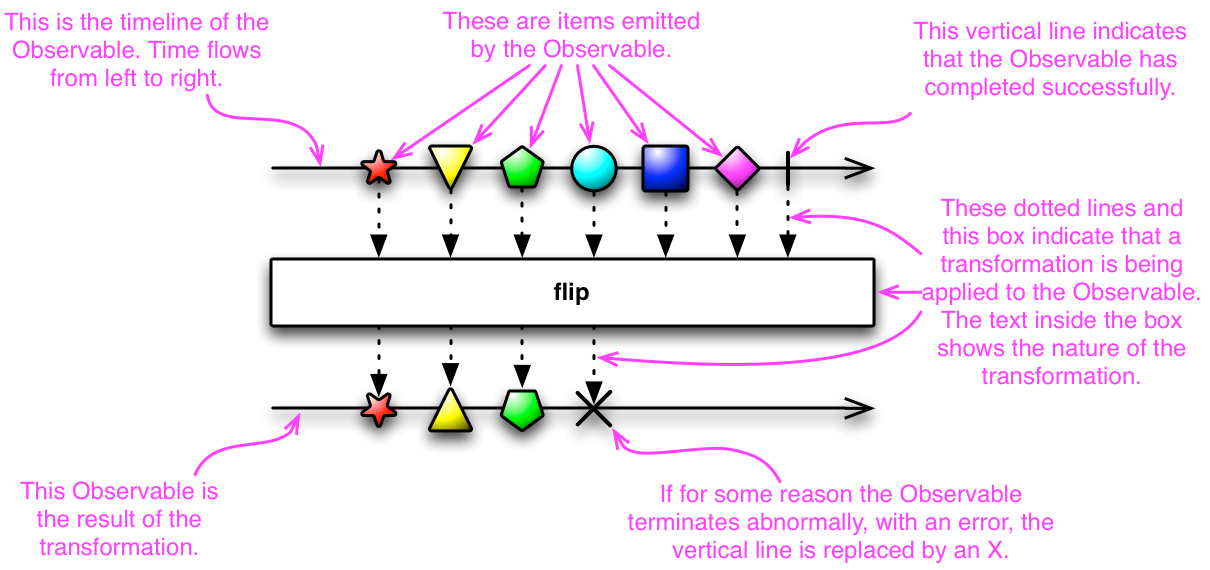
\includegraphics[width=\textwidth]{legend.png}
  \end{block}
\end{frame}

\begin{frame}[fragile]
  \frametitle{The Fall of Exception}

  \begin{minted}{java}
    public interface Observer<T> {
      void onSubscribe(@NonNull Disposable d);
      void onNext(@NonNull T t);
      void onError(@NonNull Throwable e);
      void onComplete();
    }
  \end{minted}
\end{frame}

\section{The Monadic Way: Maybe}

\begin{frame}
  \frametitle{The Monadic Way}

  \begin{block}{Monad}
    A monad is an endofunctor (a functor mapping a category to itself), together with two natural transformations.
  \end{block}
\end{frame}

\begin{frame}[fragile]
  \frametitle{The Monadic Way: Maybe}
  \begin{minted}{java}
    return a.f().g().h();
  \end{minted}
\end{frame}

\begin{frame}[fragile]
  \frametitle{The Monadic Way: Maybe}
  \begin{minted}{java}
    B b = null;
    if (a != null) {
      b = a.f();
    }
    C c = null;
    if (b != null) {
      c = b.g();
    }
    D d = null;
    if (c != null) {
      d = c.h();
    }
    return d;
  \end{minted}
\end{frame}

\begin{frame}[fragile]
  \frametitle{The Monadic Way: Maybe}
  \begin{minted}{java}
    <U,T> U andThen(T x, Function<U,T> f) {
      if (x == null) {
        return null;
      } else {
        return f(x);
      }
    }

    return andThen(andThen(andThen(a, x->x.f()), x->x.g()), x->x.h());
  \end{minted}
\end{frame}

\begin{frame}[fragile]
  \frametitle{The Monadic Way: Maybe}
  \begin{minted}{java}
    class Maybe<T> {
      T v;

      static public <U> Maybe<U> of(U x) {
        return (x == null) ? Maybe<U>() : Maybe<U>(x);
      }

      public <U> Maybe<U> andThen(Function<Maybe<U>,T> f) {
        return (v == null) ? Maybe<U>() : f(v);
      }
    }

    return Maybe::of(a)
        .andThen(x->Maybe::of(x.f()))
        .andThen(x->Maybe::of(x.g()))
        .andThen(x->Maybe::of(x.h()));
  \end{minted}
\end{frame}

\section{The Rust Way: Result}

\begin{frame}[fragile]
  \frametitle{The monadic way: Result}
  \begin{minted}{rust}
    enum Result<T, E> {
      Ok(T),
      Err(E),
    }

    let f = File::open("hello.txt");
    let f = match f {
        Ok(file) => file,
        Err(error) => {
            panic!("There was a problem opening the file: {:?}", error)
        },
    };
  \end{minted}
\end{frame}

\begin{frame}[fragile]
  \frametitle{The monadic way: Result}
  \begin{minted}{rust}
    return Ok(a)
        .and_then(|x| {x.resulted_f();})
        .and_then(|x| {x.resulted_g();})
        .and_then(|x| {x.resulted_h();});
  \end{minted}
\end{frame}

\begin{frame}[fragile]
  \frametitle{The rust way: Result}
  \begin{minted}{rust}
    macro_rules! try {
      ($expr:expr) => (match $expr {
        $crate::result::Result::Ok(val) => val,
        $crate::result::Result::Err(err) => {
          return $crate::result::Result::Err(err)
        }
      });
    }
    
    let b = try!(a.resulted_f());
    let c = try!(b.resulted_g());
    let d = try!(c.resulted_h());
    return d;
  \end{minted}
  %$
\end{frame}

\begin{frame}[fragile]
  \frametitle{The rust way: Result}
  \begin{minted}{rust}
    let b = a.resulted_f()?;
    let c = b.resulted_g()?;
    let d = c.resulted_h()?;
    return d;
  \end{minted}
\end{frame}

\section{Conclusion}

\begin{frame}
  \frametitle{Conclusion}
  \begin{block}{~}
    \begin{itemize}
    \item Challenge of error handling
    \item Exception: its rise and its fall
    \item Other ways:
      \begin{itemize}
      \item the way of RxJava
      \item the monadic way
      \item the way of Rust
      \end{itemize}
    \end{itemize}
  \end{block}
\end{frame}

\begin{frame}
  \frametitle{}
  \begin{center}
    \Huge
    Questions?
  \end{center}
\end{frame}

\end{document}
